\documentclass[10pt]{beamer}

\usetheme[progressbar=frametitle]{metropolis}
\usepackage{appendixnumberbeamer}

\usepackage[autoplay]{animate}
\usepackage{graphicx}
\usepackage{subcaption}

\usepackage{booktabs}
\usepackage[scale=2]{ccicons}

%\usepackage{pgfplots}
%\usepgfplotslibrary{dateplot}

\usepackage{xspace}

\newcommand\blfootnote[1]{%
  \begingroup
  \renewcommand\thefootnote{}\footnote{#1}%
  \addtocounter{footnote}{-1}%
  \endgroup
}

\setbeamercolor{normal text}{bg=white}
\newcommand{\themename}{\textbf{\textsc{metropolis}}\xspace}

\title{Tmux}
\subtitle{\underline{\textbf{T}}erminal \underline{\textbf{mu}}ltiple\underline{\textbf{x}}or}
\date{\today}
\date{}
\author{Simon Rydell}
\institute{Systecon}
% \titlegraphic{\hfill\includegraphics[height=1.5cm]{logo.pdf}}

\begin{document}

\begin{frame}
\titlepage
\end{frame}

%\maketitle
% 
\begin{frame}{Hello World in tmux}
% First row
    \begin{columns}[c]
        \column{3in}
        \begin{figure}[h!]
            \centering
            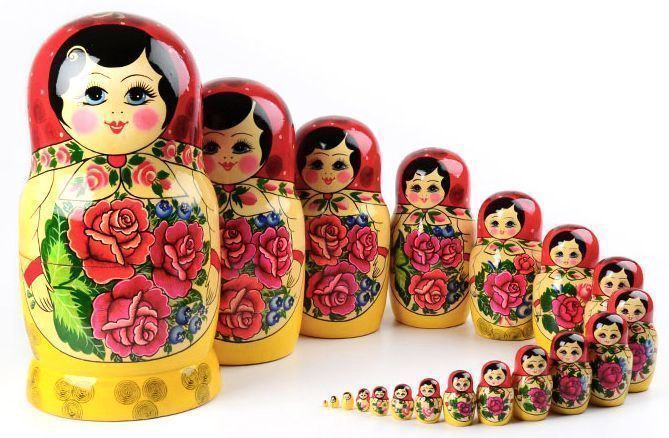
\includegraphics[width=1\textwidth]{../figures/russianDoll.jpeg}
        \end{figure}
        \column{1.5in}
        \begin{itemize}
            \item Random and self avoiding walks
            \item Spin lattices
            \item Dual transformations
            \item Geometric properties
            \item Ising, XY
        \end{itemize}
    \end{columns}
    \blfootnote{bit.ly/2qGMGnR}
\end{frame}

% 
\begin{frame}{Table of contents}
    \setbeamertemplate{section in toc}[sections numbered]
    \tableofcontents[hideallsubsections]
    \blfootnote{bit.ly/2qGMGnR}
\end{frame}


% The term fractal dimension was coined by Mandelbrot in 1975 where the dimension of some object is not limited to that of whole numbers, but can be any real positive number. When many of us think of fractals we may think of self-similar fractals such as the Koch curve or the Sierpinski triangle, but this is overly restrictive as we shall see.
\section{Ways of defining fractal dimension}


% Let's start with the example of a square and the Sierpinski triangle. Each square can be divided into four identical squares, only scaled down by a factor of one half. The Sierpinski triangle can be divided into thirds, each with the length of one half the original triangle. {Switch slide}
% Now think of the square as being made of sheet metal, and the triangle as a metal mesh. Then the mass of the square is scaled down by one fourth, while the mass of the triangle by one third. {Switch slide}
% So one way to define the dimension is as the answer to the question, if I scale my object by some factor s, then the mass of that object is scaled by s to the power d, which we call the dimension.
% Applying this logic to the Sierpinski triangle, we scale the linear length by one half, and since it's self similar, the mass goes down by one third, giving the dimension log_2 (3) = 1.585 {Switch slide}
% This way of scaling the object and fitting its scaled down version into itself is called the self similarity dimension. But what about a disk? When scaled by a factor of two, its mass scales by a factor of four, but there is no obvious way of fitting four smaller disks into a larger one. 
% So we approximate. One way of doing so is to use the box counting method. {Switch slide}

\begin{frame}{Scaling Mass}
% First row
    \begin{columns}[c]
        \column{1.5in}
        Here was a figure
    \column{1.5in}
                Here was a figure
    \end{columns}
% Second row
    \begin{columns}[c]
        \column{1.5in}
            \begin{align*}
%                L &\rightarrow \frac{1}{2} L \\
%                \left (\frac{1}{2} \right )^d M &= \frac{1}{4} M \\
%                d &= 2
            \end{align*}
        \column{1.5in}
            \begin{align*}
%                L &\rightarrow \frac{1}{2} L \\
%                \left (\frac{1}{2} \right )^d M &= \frac{1}{3} M \\
%                d &= \log_2 (3) \\ &\approx 1.585
            \end{align*}
    \end{columns}
    \blfootnote{bit.ly/2qGMGnR}
\end{frame}

\begin{frame}{Scaling Mass}
% First row
    \begin{columns}[c]
        \column{1.5in}
                Here was a figure
    \column{1.5in}
                Here was a figure
    \end{columns}
% Second row
    \begin{columns}[c]
        \column{1.5in}
            \begin{align*}
                L &\rightarrow \frac{1}{2} L \\
%                \left (\frac{1}{2} \right )^d M &= \frac{1}{4} M \\
%                d &= 2
            \end{align*}
        \column{1.5in}
            \begin{align*}
                L &\rightarrow \frac{1}{2} L \\
%                \left (\frac{1}{2} \right )^d M &= \frac{1}{3} M \\
%                d &= \log_2 (3) \\ &\approx 1.585
            \end{align*}
    \end{columns}
    \blfootnote{bit.ly/2qGMGnR}
\end{frame}

\begin{frame}{Scaling Mass}
% First row
    \begin{columns}[c]
        \column{1.5in}
                Here was a figure
    \column{1.5in}
                Here was a figure
    \end{columns}
% Second row
    \begin{columns}[c]
        \column{1.5in}
            \begin{align*}
                L &\rightarrow \frac{1}{2} L \\
                \left (\frac{1}{2} \right )^d M &= \frac{1}{4} M \\
                d &= 2
            \end{align*}
        \column{1.5in}
            \begin{align*}
                L &\rightarrow \frac{1}{2} L \\
                \left (\frac{1}{2} \right )^d M &= \frac{1}{3} M \\
                d &= \log_2 (3) \\ &\approx 1.585
            \end{align*}
    \end{columns}
    \blfootnote{bit.ly/2qGMGnR}
\end{frame}

% It divides the graph into smaller and smaller squares, called boxes in which we can count how many is needed to cover the object. The idea is that the number of boxes needed, will scale as one over the box length, epsilon, raised to the power of the dimension. {Switch slide}
% This way, if the limit when the length of these boxes goes to zero. exists, the dimension is well defined. It's essentially approximating the integral of the object! {Switch slide}
\begin{frame}{Box Counting Method}
% First row
    \begin{columns}[c]
        \column{1.5in}
                Here was a figure
        \column{1.5in}
            \begin{align*}
                N &\sim \frac{1}{\epsilon^d} \\
%                d &= \lim_{\epsilon \to 0} \frac{\ln N(\epsilon)}{\ln 1 / \epsilon}
            \end{align*}
    \end{columns}
    \blfootnote{bit.ly/2qGMGnR}
\end{frame}

\begin{frame}{Box Counting Method}
% First row
    \begin{columns}[c]
        \column{1.5in}
                Here was a figure
        \column{1.5in}
            \begin{align*}
                N &\sim \frac{1}{\epsilon^d} \\
                d &= \lim_{\epsilon \to 0^+} \frac{\ln N(\epsilon)}{\ln 1 / \epsilon}
            \end{align*}
    \end{columns}
    \blfootnote{bit.ly/2qGMGnR}
\end{frame}


% I've spoken about mass here as a loose term. What we really need to rigourously define this property is a mathematical measure. This is the Hausdorff measure of some object A, which is defined as the smallest cover of A by balls of at most diameter delta.
% Now, if there exists a smallest d, such that the limit is finite, then for all larger d, the limit goes to 0. {Switch slide}
% We define this smallest d to be the Hausdorff dimension of A.
% This coincides with the box dimension if the open set condition is fulfilled, and it is discussed a little further in the thesis.
\begin{frame}{Hausdorff Dimension}
    \begin{align*}
        \mathcal{H}_d (A) &= \lim_{\delta \to 0} \inf \left \{ \sum_{B \in \mathcal{B}} \left ( \text{diam}(B) \right)^d \right \} \\
        \text{dim}_H (A) &= \inf \{ d > 0 : \mathcal{H}_d (A) = 0 \}
    \end{align*}
    \blfootnote{bit.ly/2qGMGnR}
\end{frame}

% Next I'm going to talk about an overview of what algorithms were used in the simulations
\section{Algorithms for Working with Graph Patterns}

% The idea with the worm algorithm is to simulate spin, or more generally, graph configurations in order to sample the partition function. 
% This is done via metropolis steps and thus ensures that it adheres to detailed balance. 
% Intuitively, the ‘worm’ part can be seen as a ‘magic marker’ that can add or remove a connection between two sites.
% This way the marker draws patterns onto a lattice that corresponds to a configuration. In this thesis we are only concerned with whenever the worm reaches the same lattice site that it started on, forming loops, or clusters. And in particular we are interested in the largest of these clusters. {Switch slide}
\begin{frame}{Worm Algorithm}
    \begin{columns}[c]
        \begin{column}{0.4\textwidth}
            \begin{enumerate}[$\bullet$]
                \item Graph configurations
                \item Metropolis steps
            \end{enumerate}
        \end{column}
        \begin{column}{0.7\textwidth}  %%<--- here
                    Here was a figure
        \end{column}
    \end{columns}
    \blfootnote{bit.ly/2qGMGnR}
\end{frame}

% When a suitable number of loops have been formed, the largest cluster need to be identified. For this a labeling algorithm named after two phycisists called Hoshen and Kopelman was used. It takes a raster scan of the graph and labels the clusters recursively.
% If only the scaling dimension was of interest, the simulation could be sampled from here, but for the box dimension, the graph needs to be divided into smaller and smaller boxes. Here I utilized that all graphs simulated in this thesis had the linear system size of 2^n for some integer n. Therefore I could recursively divide each dimension in factors of 2. So for example, a 2D square would be divided into 4 squares, and a 3D cube into 8 smaller cubes and so on. {Switch slide}
\begin{frame}{Labeling and Dividing the Graph}
    \begin{columns}[c]
        \begin{column}{0.4\textwidth}
            \begin{enumerate}[$\bullet$]
                \item Hoshen-Kopelman Algorithm
                \item Graph Dividing
            \end{enumerate}
        \end{column}
        \begin{column}{0.6\textwidth}  %%<--- here
                    Here was a figure
        \end{column}
    \end{columns}
    \blfootnote{bit.ly/2qGMGnR}
\end{frame}

% The first model I used, was the familiar Ising model. First I will talk about how to relate this model with the Worm algorithm via a so called loop expansion and then I will discuss some results {Switch slide}
\section{Ising Model}

% The idea is to expand the ising partition to these sums over pairs of spins. The outer sum, is a collection of sums over each spin S_i over -1 and +1. The sum subscript of the inner sums represent the contiguous length of each link. {Switch slide}
\begin{frame}{Ising Loop Expansion}
    \begin{equation*}
        Z &\propto  \sum_{\{S\}} \left ( 1 + \tanh(K) \sum_{l = 1} S_i S_j + \tanh^2(K) \sum_{l = 2} (S_i S_j)(S_{i'} S_{j'}) + \ldots \right)
    \end{equation*}
    \blfootnote{bit.ly/2qGMGnR}
\end{frame}

% Here we can see the link structure in between sites. Since the partition function includes a sum over all states of each individual spin, in this case +1 and -1, only the terms with a full loop will survive, since these only have terms such as $S_i^2$. {Switch slide}
\begin{frame}{Ising Loop Expansion}
        Here was a figure
\blfootnote{bit.ly/2qGMGnR}
\end{frame}

% Given enough sampling, a physical system will emerge. This can then be divided as per the discussed scaling method.  The result is here compared to the theoretical value given by Loewner expansion. So we can see a somewhat close approximation. {Switch slide}
\begin{frame}{Scaling Dimension Ising Cluster}
            Here was a figure
\footnotesize [1] B. Duplantier, Conformally Invariant Fractals and Potential Theory, Physical Review Letters 84, 1363 (2000).
\\
    \blfootnote{bit.ly/2qGMGnR}
\end{frame}

% If we instead use the box counting method, the result can be seen in this plot. The x-axis here shows the relative size of the box division, so a relative size of 1 would be the whole system. {Switch slide}
\begin{frame}{Box Dimension Ising Cluster}
            Here was a figure
\footnotesize [1] B. Duplantier, Conformally Invariant Fractals and Potential Theory, Physical Review Letters 84, 1363 (2000).
\\
    \blfootnote{bit.ly/2qGMGnR}
\end{frame}


% We can see that both the box- as well as the scaling dimension give a result close to the theoretical value, showed here in green. Peculiar enough, the clusters has almost the same hausdorff dimension as a self avoiding walk, shown here in yellow. This suggest some similarities between the structure of the SAW and the ising clusters
\begin{frame}{Comparison of Dimensions $2D$ Ising}
          Here was a figure
    \blfootnote{bit.ly/2qGMGnR}
\end{frame}

% If we further examine a cluster on a 128^2 ising lattice we can see the familiar `swollen' structure in the loop. The only visible difference here is that `twisted loops' are allowed as it doesn't cost any energy to create them in the worm algorithm and we can see these on multiple places on the perimiter of the graph.
% To further get intuition about how this process is done, I created a small animation of a 2D Ising lattice. From the point where some clusters have formed, we identify the largest cluster with the Hoshen Kopelman algorithm and the lattice is divided into smaller and smaller boxes.
\begin{frame}{Largest Ising Loop on a $128^2$ Lattice}
%    \begin{figure}[h!]
%        \centering
%            \includegraphics[width=0.8\textwidth]{figures/largest_cluster_testing_nolattice.pdf}
%    \end{figure}
            Here was a figure
\blfootnote{bit.ly/2qGMGnR}
\end{frame}

\begin{frame}{$2D$ Ising Animation}
    % TODO: Uncomment
        Here was a figure
     \blfootnote{bit.ly/2qGMGnR}
\end{frame}

% Next I will talk about the XY model, often called the xy rotor model since the spins can rotate in a plane. 
\section{XY Model}

% The XY model allows spin to rotate around some axis in a plane. Giving a Hamiltonian as a function of the difference in angle in this plane. 
% Therefore we get the 2 pi symmetric partition function, that can be fourier transformed as
\begin{frame}{XY Loop Expansion - Hamiltonian \& Partition Function}
    \begin{align*}
        H &= - J \sum_{\langle ij \rangle} \cos(\theta_i - \theta_j) \\
        Z &= \prod_i \int \frac{\mathrm d \theta_i}{2 \pi} \prod_{\langle ij \rangle} e^{K  \cos(\theta_i - \theta_j)}
    \end{align*}
    \blfootnote{bit.ly/2qGMGnR}
\end{frame}

% Where lower case j here is the fourier coefficients summed over the nearest neighbours. Expanding this integral shows
\begin{frame}{XY Loop Expansion}
    \begin{align*}
        Z &\sim \int \frac{\mathrm d \theta_i}{2 \pi} e^{i \sum_{\langle ij \rangle} j_{\langle ij \rangle} (\theta_i - \theta_j)} \\
        & \sim \delta_{0, \sum_{\langle ij \rangle} j_{\langle ij \rangle}}
    \end{align*}
    \blfootnote{bit.ly/2qGMGnR}
\end{frame}

% that the sum of the links from each site to its neighbours must be zero. We can convince ourselves that this in turn means that the links together will form loops.
% This does add a bit of complexity compared to the Ising loop expansion. Here each link can have either positive or negative values, so we interpret this as direction. So instead of connecting site a and b, we connect site a to b with some weight w, giving something like this...
%\begin{frame}{XY Loop Expansion}

%\end{frame}

% where the size of the arrow is related to the magnitute of the current on that link. 
%\begin{frame}{XY Loop expansion}
%    \begin{figure}[h!]
%        \centering
%            \includegraphics[width=0.8\textwidth]{figures/%percolatingFlux.pdf}
%    \end{figure}
%\end{frame}

% So here is a completely blank system, where no configurations have been formed. As you can see there are periodic boundary conditions and the size of each arrow represents the weight between the two sites.
\begin{frame}{$3D$ XY Animation - $4^3$ system}
        Here was a figure
   \blfootnote{bit.ly/2qGMGnR}
\end{frame}

% To simplify the acceptance probability I used the Villain approximation where the energy is simply the sum of these fourier coefficients squared.
% In this approximation, the notion of temperature is exchanged for one over temperature, leading to a shift in the critical temperature. One way to find the new Tc is to examine the superfluid density of the system, and notice that it is proportional to an easily measurable quantity called the winding number
\begin{frame}{Villain Model}
    \begin{equation*}
        E = \frac{1}{2} \sum_i j_i^2
    \end{equation*}
    \begin{align*}
        \lim_{\beta \to \infty} \beta_d = 0 \qquad \lim_{\beta \to 0} \beta_d = \infty
    \end{align*}
    \blfootnote{bit.ly/2qGMGnR}
\end{frame}

% Where rho_s is the superfluid density and W_mu is the winding number in the mu direction. Intuitively, this says something about how many times the current percolates in the mu direction.
% We can then plot the winding number for a range of temperatures and system sizes to look for an intersection where the superfluid density goes to zero.
\begin{frame}{Winding Number}
    \begin{equation*}
        \rho_s = L^{2 - d} T \langle W_\mu^2 \rangle 
    \end{equation*}
    \blfootnote{bit.ly/2qGMGnR}
\end{frame}

% which is done here. The darker the blue, the larger the system is, and the intersection showed in red is taken as the weighted average of the intersections of all system sizes.
% Now that the critical temperature is known, the fractal dimension of the clusters can be examined.
\begin{frame}{Winding Number}
            Here was a figure
    \blfootnote{bit.ly/2qGMGnR}
\end{frame}

% In the year 2000 Hove, Mo and Sudbo published an article with the result of 2.287 for the Hausdorff dimension of an XY system. This was refuted by Prokof'ev and Svistunov in 2005 with a comment, arguing that Hove, Mo and Sudbo made a mistake in their self-similar expression for the dimension. Their result clearly differs from Hove, Mo and Sudbo's.
% Recreating this with the box dimension...
\begin{frame}{$3D$ XY Model Hausdorff Dimension}
    \begin{align*}
        \bullet \ &\text{Hove, Mo and Sudbo (2000):}\ &D_H = 2.287 \pm 4 \cdot 10^{-3} [1] \\
        \bullet \ &\text{Prokof'ev and Svistunov Comment (2006):} \ &D_H = 1.765 \pm 2 \cdot 10^{-3} [2]
    \end{align*}
    \blfootnote{bit.ly/2qGMGnR}
        

\footnotesize [1] J. Hove, S. Mo and A. Sudbø, Hausdorff Dimension of Critical Fluctuations in Abelian Gauge Theories, Physical Review Letters 85, 2368 (2000).

\footnotesize [2] N. Prokofev and B. Svistunov, Comment on Hausdorff Dimension of Critical Fluctuations in Abelian Gauge Theories”, Physical Review Letters 96 (2006).

\end{frame}

% ...clearly favours Prokof'ev and Svistunov with the value from this thesis being 1.77468. Here Prokof'evs results is labeled D_H^P, while Sudbo's D_H^S. In 2006, Sudbo replied, and the issue concerned if the interactions between the loops are local or not. In this thesis the interactions are completely local, and it does not necessarily correspond to the same fractal dimension.
\begin{frame}{Box Counting Method $3D$ XY}
           Here was a figure
    \blfootnote{bit.ly/2qGMGnR}
\end{frame}

% Here is a final comparison without the extra data from my simulations. Now to get a bit more intuition about how these systems actually form I will show two animations, one of a smaller system where each step in the worm algorithm can be seen clearly, and one of the largest cluster of a system more closely to those I've actually measured on.
\begin{frame}{Comparison of Dimensions $3D$ XY}
            Here was a figure
    \blfootnote{bit.ly/2qGMGnR}
\end{frame}


% So here is a completely blank system, where no configurations have been formed. As you can see there are periodic boundary conditions and the size of each arrow represents the weight between the two sites.
%\begin{frame}{$3D$ XY Animation - $4^3$ system}
% TODO: Uncomment
  % \animategraphics[width=\linewidth,loop]{10}{figures/3dxy_animation}{}{}
%\end{frame}

% So here is a 64^3 system where the sites that are linked in the largest cluster is highlighted in red. So this lattice would then be divided into boxes and checked what the minimal cover is.
\begin{frame}{$3D$ XY Animation - Largest cluster}
% TODO: Uncomment
        Here was a figure
           \blfootnote{bit.ly/2qGMGnR}
\end{frame}

% Finally, here is a small summary of the major results in this thesis. Thank you. Any questions?
\begin{frame}{Summary}
    \begin{table}
        \parbox{.45\linewidth}{
            \centering
            \begin{tabular}{l|l}
                               & $D_H$          \\ \hline
                Box            & $1.35193(5)$   \\ \hline
                Scaling        & $1.386(2)$      \\ \hline
                $D_H^G$        & $1.375$ [1]       \\ \hline
                SAW            & $1.33$                              
            \end{tabular}
            \caption{$2D$ Ising}
        }
        \hfill
        \parbox{.45\linewidth}{
            \centering
            \begin{tabular}{l|l}
                            & $D_H$           \\ \hline
                Box         & $1.77468(4)$    \\ \hline
                Prokof'ev   & $1.765(2)$ [2]      \\ \hline
                Sudbo       & $2.287(2)$ [3] 
            \end{tabular}
            \caption{$3D$ XY}
        }
    \end{table}
    \blfootnote{bit.ly/2qGMGnR}

\footnotesize [1] B. Duplantier, Conformally Invariant Fractals and Potential Theory, Physical Review Letters 84, 1363 (2000).
    
\footnotesize [2] N. Prokofev and B. Svistunov, Comment on Hausdorff Dimension of Critical Fluctuations in Abelian Gauge Theories”, Physical Review Letters 96 (2006).

\footnotesize [3] J. Hove, S. Mo and A. Sudbø, Hausdorff Dimension of Critical Fluctuations in Abelian Gauge Theories, Physical Review Letters 85, 2368 (2000).

\end{frame}


\appendix
% --------------- Backup slides ---------------

% --------------- Ising ---------------
\begin{frame}[fragile]{Extra slides: Box Dimension $64^2$ Ising}
            Here was a figure
    \blfootnote{bit.ly/2qGMGnR}
\end{frame}

\begin{frame}[fragile]{Extra slides: Susceptibility $2D$ Ising}
          Here was a figure
    \blfootnote{bit.ly/2qGMGnR}
\end{frame}

\begin{frame}[fragile]{Extra slides: Largest Ising cluster}
        Here was a figure
    \blfootnote{bit.ly/2qGMGnR}
\end{frame}

\begin{frame}[fragile]{Extra slides: Self avoiding walk}
        Here was a figure
    \blfootnote{bit.ly/2qGMGnR}
\end{frame}

% --------------- Graph Dividing ---------------

\begin{frame}[fragile]{Extra slides: Graph Dividing Algorithm}
        Here was a figure
    \blfootnote{bit.ly/2qGMGnR}
\end{frame}

\begin{frame}[fragile]{Extra slides: Graph Dividing Algorithm}
        Here was a figure
    \blfootnote{bit.ly/2qGMGnR}
\end{frame}


\end{document}